\chapter{Results}

\section{Overview}
This chapter shows the results obtained after performing computations on the datasets. The plot and heat maps are generated to get a better visualization of the results obtained.

\section{Qualitative Analysis}
The following are the results we obtain in the form of graph for Rwanda and heat maps of countries Rwanda, Mozambique, Nigeria and Madagascar. These are the results obtained using the model mentioned in the report.


\begin{figure}[h!]
\centering
  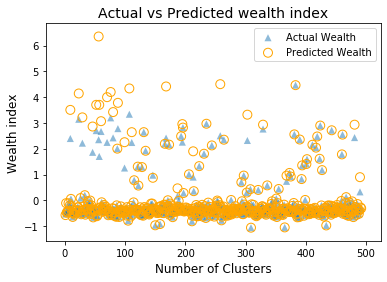
\includegraphics[width=8cm]{setup/img/actvspredwlth.png}
  \newline
  \caption{Actual wealth vs predicted wealth of Rwanda.}
  \label{fig3}
  \centering
\end{figure}




\begin{figure*}[!ht]
    \hspace{3cm} Input: Sample Day-time satellite images
    \newline
    \newline
     \centering
     %----day-time inputs--------------
     \begin{subfigure}[t]{0.22\textwidth}
         \centering
         \setlength{\unitlength}{0.1\textwidth}
         \begin{picture}(10,9)
         \put(0,0){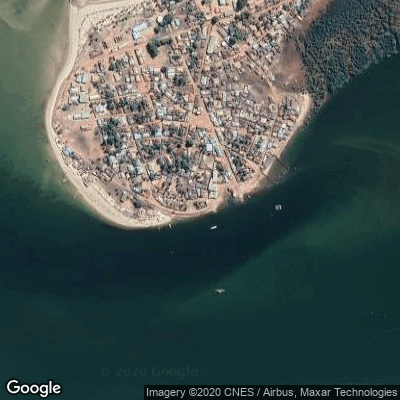
\includegraphics[trim={0.5cm, 0cm, 0cm, 2.25cm}, clip, width=\columnwidth]{setup/img/Madagascar_day.png}}
         \color{yellow}
         \put(0.0,0.5){{-16.104434,45.328354}}
         \end{picture}
        %  \caption{Madagascar}
         \label{fig:y equals x}
     \end{subfigure}
     \hfill
     \begin{subfigure}[t]{0.22\textwidth}
         \centering
         \setlength{\unitlength}{0.1\textwidth}
         \begin{picture}(10,9)
         \put(0,0){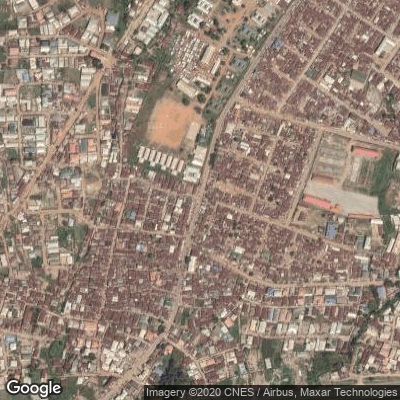
\includegraphics[trim={0.5cm, 0cm, 0cm, 2.25cm}, clip, width=\columnwidth]{setup/img/nigeria_day.png}}
         \color{yellow}
         \put(0.0,0.5){{9.145108,7.316459}}
        %  \caption{Nigeria}
         \end{picture}
         \label{fig:five over x}
     \end{subfigure} 
     \hfill
    \begin{subfigure}[t]{0.22\textwidth}
         \centering
         \setlength{\unitlength}{0.1\textwidth}
         \begin{picture}(10,9)
         \put(0,0){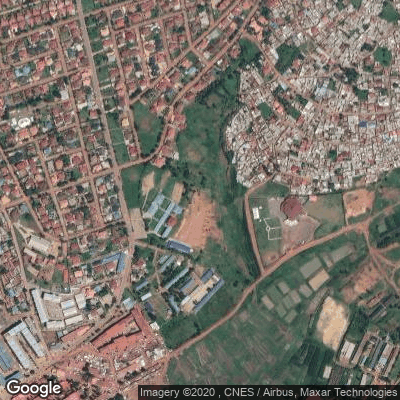
\includegraphics[trim={0.5cm, 0cm, 0cm, 2.25cm}, clip, width=\columnwidth]{setup/img/Rwanda_day.png}}
         \color{yellow}
         \put(0.0,0.5){{-1.920349,30.074494}}
         \end{picture}
        %  \caption{Rwanda}
         \label{fig:five over x}
     \end{subfigure}
     \hfill
     \begin{subfigure}[t]{0.22\textwidth}
         \centering
         \setlength{\unitlength}{0.1\textwidth}
         \begin{picture}(10,9)
         \put(0,0){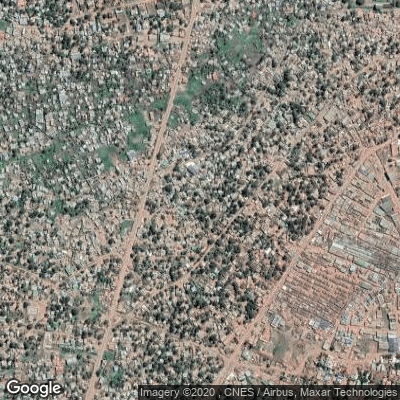
\includegraphics[trim={0.5cm, 0cm, 0cm, 2.25cm}, clip, width=\columnwidth]{setup/img/Mozambique_day.png}}
         \color{yellow}
         \put(0.0,0.5){{-19.13401772,33.48299979}}
         \end{picture}
        %  \caption{Mozambique}
         \label{fig:three sin x}
     \end{subfigure}
     \hfill

    %----predicted heat-map--------------
    

     \centering
     \begin{subfigure}[t]{0.22\textwidth}
         \centering
         \setlength{\unitlength}{0.1\textwidth}
         \begin{picture}(10,9)
         \put(0,0){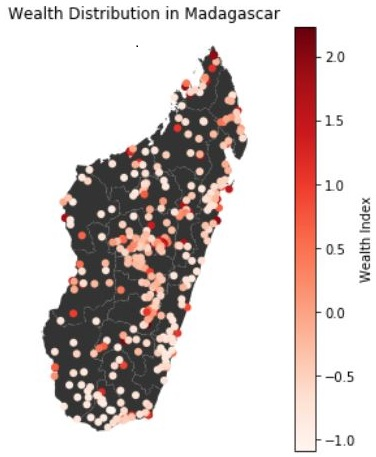
\includegraphics[trim={0.5cm, 0.5cm, 2.0cm, 1.0cm}, clip, height=3.6cm]{setup/img/Madagascar.JPG}}
         \color{yellow}
         \put(1.5,6.3){\vector(1,2){2.45}}
         \end{picture}
         %\caption{Madagascar}
         \label{fig:y equals x}
     \end{subfigure}
     \hfill
     \begin{subfigure}[t]{0.22\textwidth}
         \centering
         \setlength{\unitlength}{0.1\textwidth}
         \begin{picture}(10,9)
         \put(0,0){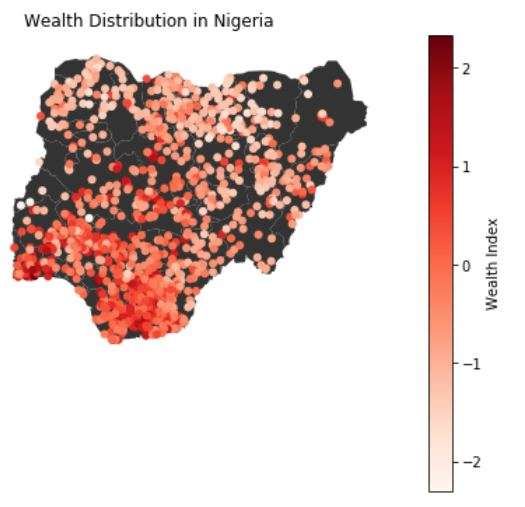
\includegraphics[trim={0.1cm, 3.0cm, 2.5cm, 1.0cm}, clip, height=3.6cm]{setup/img/Nigeria.JPG}}
         \color{yellow}
         \put(4,4.5){\vector(1,2){3.35}}
         \end{picture}
         %\caption{Nigeria}
         \label{fig:five over x}
     \end{subfigure} 
     \hfill
    \begin{subfigure}[t]{0.22\textwidth}
         \centering
         \setlength{\unitlength}{0.1\textwidth}
         \begin{picture}(10,9)
         \put(0,0){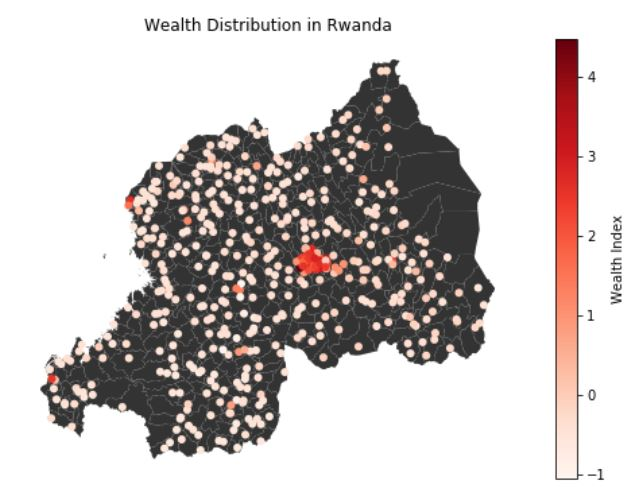
\includegraphics[trim={0.5cm, 0.5cm, 2.5cm, 1.0cm}, clip, height=3.6cm]{setup/img/rwanda.JPG}}
         \color{yellow}
         \put(6,4.5){\vector(1,2){3.35}}
         \end{picture}
         %\caption{Rwanda}
         \label{fig:five over x}
     \end{subfigure}
     \hfill
     \begin{subfigure}[t]{0.25\textwidth}
         \centering
         \setlength{\unitlength}{0.1\textwidth}
         \begin{picture}(10,9)
         \put(0,0){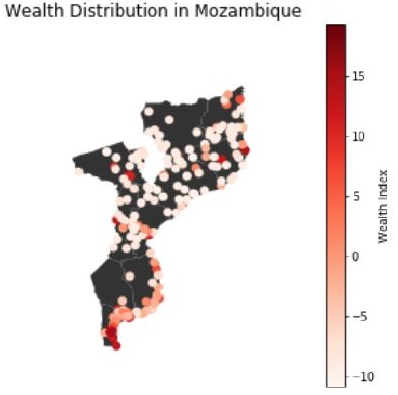
\includegraphics[trim={0.5cm, 0.5cm, 0.1cm, 1.5cm}, clip, height=3.6cm]{setup/img/Mozambique.JPG}}
         \color{yellow}
         \put(2.5,3.80){\vector(1,2){3.05}}
         \end{picture}
         %\caption{Mozambique}
         \label{fig:three sin x}
     \end{subfigure}
     \hfill

     %---- actual heat-map--------------
     \hspace{3cm} Output: Predicted wealth index heat map
     \newline \newline
     \newline
     \begin{subfigure}[t]{0.22\textwidth}

         \centering
         \setlength{\unitlength}{0.1\textwidth}
         \begin{picture}(10,9)
         \put(0,0){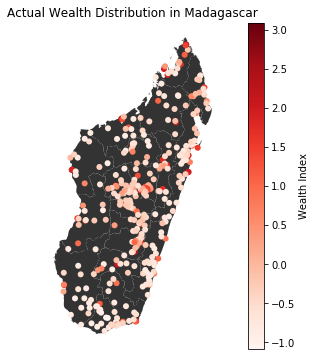
\includegraphics[trim={0.5cm, 0.5cm, 2.5cm, 1.5cm}, clip, height=3.6cm]{setup/img/Act_Madagascar.png}}

         \end{picture}
         \caption{Madagascar}
         \label{fig:y equals x}
     \end{subfigure}
     \hfill
     \begin{subfigure}[t]{0.22\textwidth}
         \centering
         \setlength{\unitlength}{0.1\textwidth}
         \begin{picture}(10,9)
         \put(0,0){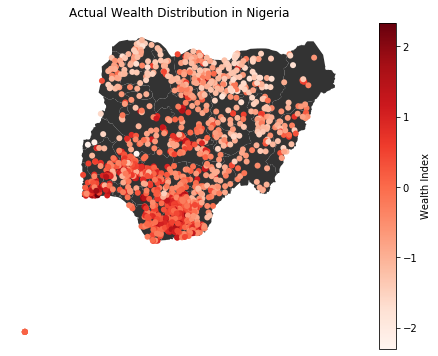
\includegraphics[trim={2.5cm, 2.5cm, 2.5cm, 1.5cm}, clip, height=3.6cm]{setup/img/Act_Nigeria.png}}
         \end{picture}
         \caption{Nigeria}
         \label{fig:five over x}
     \end{subfigure} 
     \hfill
     \begin{subfigure}[t]{0.22\textwidth}
         \centering
         \setlength{\unitlength}{0.1\textwidth}
         \begin{picture}(10,9)
         \put(0,0){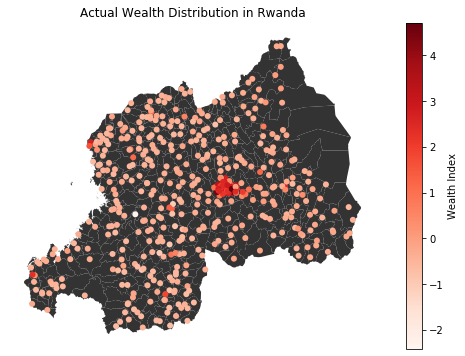
\includegraphics[trim={0.5cm, 0cm, 2.5cm, 1cm}, clip, height=3.6cm]{setup/img/Act_Rwanda.png}}

         \end{picture}
         \caption{Rwanda}
         \label{fig:five over x}
     \end{subfigure}
     \hfill
     \begin{subfigure}[t]{0.22\textwidth}
         \centering
         \setlength{\unitlength}{0.1\textwidth}
         \begin{picture}(10,9)
         \put(0,0){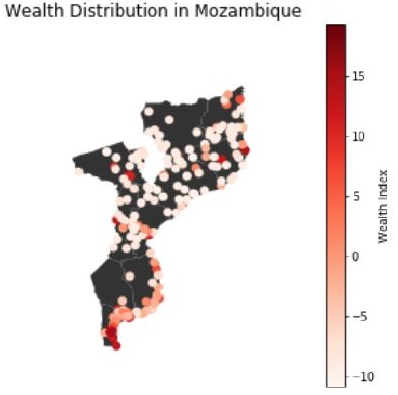
\includegraphics[trim={0.5cm, 0cm, 0cm, 1.25cm}, clip, height=3.6cm]{setup/img/Act_Mozambique.JPG}}
         
         \end{picture}
         \caption{Mozambique}
         \label{fig:three sin x}
     \end{subfigure}
     \hfill
     \newline
     \newline
     \newline
    \hspace{3cm} Actual wealth index heat map
     
     \caption{The inputs (day-time satellite images) taken from satellite CNES/Airbus of Maxar Technologies, 2019 and the predicted wealth index heat-maps of the countries: Madagascar, Nigeria, Rwanda, Mozambique. The resolution of day-time images is $400\times 400$ $dpi$.}
     \label{fig:predicted_hmap}
    
    
\end{figure*}



Fig.~\ref{fig3} compares the actual and predicted wealth index w.r.t. the number of clusters of the country, Rwanda. This scatter plot shows the difference between the original wealth and the model wealth where most of the clusters are below the $0$ wealth index. Moreover, both wealth indexes overlap at most of the clusters indicating no drastic discrepancies. Similar graphs are plotted for other countries. Fig.~\ref{fig:predicted_hmap} shows the day-time satellite images and wealth distribution in a heat map of the countries: Madagascar, Nigeria, Rwanda, and Mozambique. The day-time images here are the samples taken from medium and high-intensity categories to show human settlements of the above-mentioned countries. The corresponding night-light intensities of Madagascar, Nigeria, Rwanda, and Mozambique are $5$, $37$, $62$, and $42$ respectively. The wealth index scale differs for every country. 
